\documentclass[a4paper, fontsize = 14pt]{article}
\usepackage{hyperref}
\usepackage[warn]{mathtext}
\usepackage[english,russian]{babel}
\usepackage[utf8x]{inputenc} 
 
%математика
\usepackage[mathscr]{eucal}
\usepackage{amsmath,amsfonts,amssymb,amsthm,mathtools}
\usepackage{icomma}
\usepackage{wasysym}
\usepackage{mathrsfs}
 
%оформление текста
\usepackage{setspace}
\onehalfspacing
\usepackage{indentfirst}
\usepackage{scrextend}
 
%геометрия
\usepackage{geometry}
\geometry{left=25mm,right=25mm,
 top=25mm,bottom=30mm}
 
%графика
\usepackage{wrapfig}
\usepackage{graphicx}
\usepackage{pgfplots}
\usepackage{tikz}
\RequirePackage{caption}
\DeclareCaptionLabelSeparator{defffis}{ --- }
\captionsetup{justification=centering,labelsep=defffis}
 
%таблицы
\usepackage{array,tabularx,tabulary,booktabs} 
\usepackage{longtable}  
\usepackage{multirow} 
 
%ссылки
\usepackage{hyperref}
\usepackage{xcolor}
\definecolor{grn}{HTML}{57A14F} %зеленый
\definecolor{rd}{HTML}{E53C44} %красный 
\definecolor{bl}{HTML}{282691} %синий 
\definecolor{bbl}{HTML}{001B6C} %темно-синий
\hypersetup{		
    colorlinks=true,       	
    linkcolor=bbl,          % внутренние ссылки
    citecolor=rd,          % на библиографию
    filecolor=magenta,      % на файлы
    urlcolor=bl           %внешние источники
}
 
% Колонтитулы
\usepackage{fancyhdr} 
 	\pagestyle{fancy}
 	\renewcommand{\headrulewidth}{0.15mm}  
 	\renewcommand{\footrulewidth}{0.15mm}
 	\lfoot{МФТИ, 2021}
 	\rfoot{\thepage}
 	\cfoot{}
 	\rhead{}
 	\chead{}
 	\lhead{}
 
 
\begin{document}

\begin{center} \textbf{
Лабораторная работа №2.4.1 \\ Определение теплоты испарения жидкости \\
Мещеряков Всеволод, Б02-001, 23.03.2021}
\end{center} 

\subsection*{Введение}

В этой работе будет измеряться зависимость давления насыщенных паров от температуры, по которой будут определены теплоты испарения с помощью уравнения Клапейрона-Клаузиуса. Будут использоваться: термостат, герметический сосуд с исследуемой жидкостью, микроскоп.

\subsection*{Теоретическая справка}

Теплоту парообразования жидкости будем вычислять при помощи следствия из формулы Клапейрона-Клаузиуса (1). В ней $P$ - давление насыщенного пара при температуре $T$, $L$ - теплота испарения жидкости. Она получена из соображений, что водяной пар можно считать идеальным газом, а объем жидкости много меньше объема пара:

\begin{equation}
	L = - R \frac{d\ln(1/P)}{d(1/T)}.
\end{equation}

\subsection*{Экспериментальная установка}

\begin{figure}[hbt]\label{risI}
\center{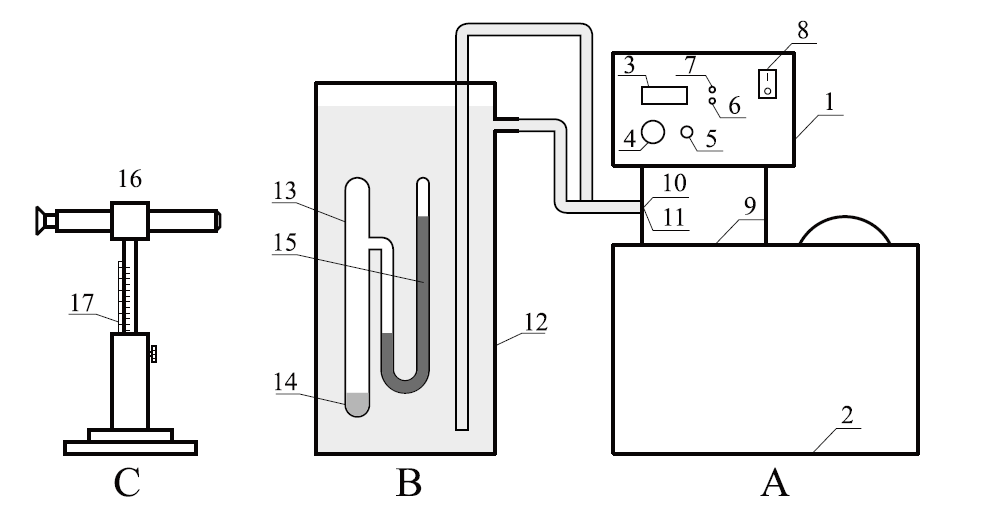
\includegraphics[scale=0.7]{lab241ris1.png}}
\caption{\textit{Схема установки}}
\end{figure}

На рисунке 1 представлена схема установки. На ней: А - термостат, В - экспериментальный прибор, С - микроскоп. Экспериментальный прибор представляет собой емкость 12, которая заполнена водой из термостата. В нее погружен прибор 13 с исследуемой жидкостью 14. Перед заполнением жидкостью прибор был откачан, так что в нем над жидкостью находится только её насыщенный пар. Рост давления пара с ростом температуры воды из термостата фиксируется по ртутному манометру 15 с помощью микроскопа 16 и штатива 17.

Недостаток этой установки состоит в том, что термостат показывает температуру воды, а не исследуемой жидкости. Поэтому при изменении температуры на $1^\circ C$ необходимо ждать 1 - 3 минуты, пока температуры выровняются.

\subsection*{Ход работы}

Включим термостат и выставим начальную температуру в $20^\circ C$. Зафиксируем давление паров. Будем продолжать измерения до $60^\circ C$ с шагом в $2^\circ C$. Результаты отразим в таблице 1 приложения. По этим данным построим графики в координатах $T$ и $P$, $1/T$ и $ln{P}$: рисунки 2 и 3 приложения. График рисунка 2 проще анализировать, поэтому воспользуемся им. 

Коэффициент наклона из формулы (1):

\begin{equation}
	\frac{L}{R}= - \frac{d ln{1/P}}{d(1/T)} \Longrightarrow L = 43.063\pm250 \, Дж/кг
\end{equation}

Так же измерим зависимость расхода от диаметра трубки. Согласно теории, он пропорционален его четвертой степени при турбулентном течении. Результаты отразим в таблице 2 и на рисунке 4 приложения.

\newpage

\subsection*{Приложение}

\begin{table}[hbt]
\centering
\caption{\textit{Зависимость перепада давления от температуры}}
\scalebox{0.9}{
\begin{tabular}{|c|c|c|c|c|}
\hline
\textbf{$T, К$} & \textbf{$dH, см$} & \textbf{$dD, см$} & \textbf{$dP, Па$} & \textbf{$\sigma_{dP}, Па$} \\ \hline
293,03          & 1,77              & 0,04              & 2330,2            & 11,7                       \\ \hline
295,04          & 1,93              & 0,13              & 2532,3            & 12,7                       \\ \hline
296,95          & 2,14              & 0,05              & 2817,1            & 14,1                       \\ \hline
299,97          & 2,63              & 0,3               & 3438,7            & 17,2                       \\ \hline
302,96          & 3,07              & 0,07              & 4041,5            & 20,2                       \\ \hline
305,07          & 3,47              & 0,11              & 4565,1            & 22,8                       \\ \hline
307,01          & 3,85              & 0,07              & 5070,1            & 25,4                       \\ \hline
309,03          & 4,31              & 0,12              & 5671,8            & 28,4                       \\ \hline
311,04          & 4,86              & 0,18              & 6391,2            & 32,0                       \\ \hline
313,04          & 5,18              & 0,04              & 6826,9            & 34,1                       \\ \hline
315,03          & 6,06              & 0,13              & 7978,5            & 39,9                       \\ \hline
317,07          & 6,6               & 0,09              & 8694,5            & 43,5                       \\ \hline
319,03          & 7,45              & 0,13              & 9811,5            & 49,1                       \\ \hline
321,02          & 8,11              & 0,05              & 10689,7           & 53,4                       \\ \hline
323,04          & 8,85              & 0,03              & 11667,4           & 58,3                       \\ \hline
325,03          & 9,94              & 0,03              & 13104,8           & 65,5                       \\ \hline
327,03          & 10,4              & 0,05              & 13709,5           & 68,5                       \\ \hline
329,02          & 12                & 0,05              & 15819,4           & 79,1                       \\ \hline
331,04          & 13,21             & 0,08              & 17412,0           & 87,1                       \\ \hline
333,02          & 14,49             & 0,08              & 19099,9           & 95,5                       \\ \hline
\end{tabular}
}
\end{table}

\begin{figure}[hbt]\label{risI}
\center{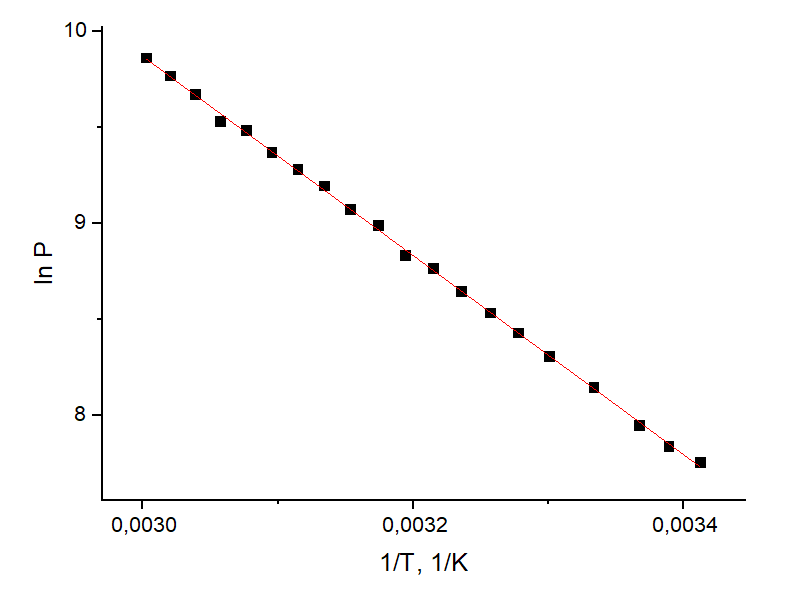
\includegraphics[scale=0.7]{lab241ris2.png}}
\caption{\textit{График зависимости в координатах $1/T$, $ln{P}$}}
\end{figure}

\begin{figure}[hbt]\label{risI}
\center{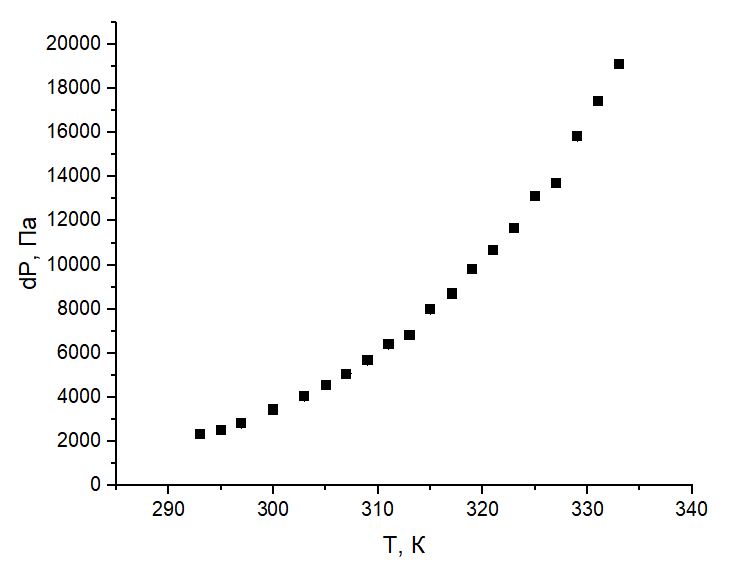
\includegraphics[scale=0.7]{lab241ris3.png}}
\caption{\textit{График зависимости в координатах $T$, $P$}}
\end{figure}


\end{document}
